\documentclass[a4paper,10pt]{article}
\usepackage[brazilian]{babel}
\usepackage[left=2.5cm,right=2.5cm,top=3cm,bottom=2.5cm]{geometry}
\usepackage{mathtools}
\usepackage{amsthm}
\usepackage{amsmath}
%\usepackage{nccmath}
\usepackage{amssymb}
\usepackage{amsfonts}
\usepackage{physics}
%\usepackage{dsfont}
%\usepackage{mathrsfs}

\usepackage{titling}
\usepackage{indentfirst}

\usepackage{bm}
\usepackage[dvipsnames]{xcolor}
\usepackage{cancel}

\usepackage{xurl}
\usepackage[colorlinks=true]{hyperref}

\usepackage{float}
\usepackage{graphicx}
%\usepackage{tikz}
\usepackage{caption}
\usepackage{subcaption}

%%%%%%%%%%%%%%%%%%%%%%%%%%%%%%%%%%%%%%%%%%%%%%%%%%%

\newcommand{\eps}{\epsilon}
\newcommand{\vphi}{\varphi}
\newcommand{\cte}{\text{cte}}

\newcommand{\N}{\mathbb{N}}
\newcommand{\Z}{\mathbb{Z}}
\newcommand{\Q}{\mathbb{Q}}
\newcommand{\R}{\vb{R}}
\newcommand{\C}{\mathbb{C}}
\renewcommand{\S}{\hat{S}}
%\renewcommand{\H}{\s{H}}

\renewcommand{\a}{\vb{a}}
\newcommand{\nn}{\hat{n}}
\renewcommand{\d}{\dagger}
\newcommand{\up}{\uparrow}
\newcommand{\down}{\downarrow}

\newcommand{\0}{\vb{0}}
%\newcommand{\1}{\mathds{1}}
\newcommand{\E}{\vb{E}}
\newcommand{\B}{\vb{B}}
\renewcommand{\v}{\vb{v}}
\renewcommand{\r}{\vb{r}}
\renewcommand{\k}{\vb{k}}
\newcommand{\p}{\vb{p}}
\newcommand{\q}{\vb{q}}
\newcommand{\F}{\vb{F}}

\newcommand{\s}{\sigma}
%\newcommand{\prodint}[2]{\left\langle #1 , #2 \right\rangle}
\newcommand{\cc}[1]{\overline{#1}}
\newcommand{\Eval}[3]{\eval{\left( #1 \right)}_{#2}^{#3}}

\newcommand{\unit}[1]{\; \mathrm{#1}}

\newcommand{\n}{\medskip}
\newcommand{\e}{\quad \mathrm{e} \quad}
\newcommand{\ou}{\quad \mathrm{ou} \quad}
\newcommand{\virg}{\, , \;}
\newcommand{\ptodo}{\forall \,}
\renewcommand{\implies}{\; \Rightarrow \;}
%\newcommand{\eqname}[1]{\tag*{#1}} % Tag equation with name

\setlength{\droptitle}{-7em}

\theoremstyle{plain}
\newtheorem{theorem}{Teorema}[section]
%\newtheorem{defi}[theorem]{Definição}
\newtheorem{lemma}[theorem]{Lema}
%\newtheorem{corol}[theorem]{Corolário}
%\newtheorem{prop}[theorem]{Proposição}
%\newtheorem{example}{Exemplo}
%
%\newtheorem{inneraxiom}{Axioma}
%\newenvironment{axioma}[1]
%  {\renewcommand\theinneraxiom{#1}\inneraxiom}
%  {\endinneraxiom}
%
%\newtheorem{innerpostulado}{Postulado}
%\newenvironment{postulado}[1]
%  {\renewcommand\theinnerpostulado{#1}\innerpostulado}
%  {\endinnerpostulado}
%
%\newtheorem{innerexercise}{Exercício}
%\newenvironment{exercise}[1]
%  {\renewcommand\theinnerexercise{#1}\innerexercise}
%  {\endinnerexercise}
%
%\newtheorem{innerthm}{Teorema}
%\newenvironment{teorema}[1]
%  {\renewcommand\theinnerthm{#1}\innerthm}
%  {\endinnerthm}
%
\newtheorem{innerlema}{Lema}
\newenvironment{lema}[1]
  {\renewcommand\theinnerlema{#1}\innerlema}
  {\endinnerlema}
%
%\theoremstyle{remark}
%\newtheorem*{hint}{Dica}
%\newtheorem*{notation}{Notação}
%\newtheorem*{obs}{Observação}


%\documentclass[../main.tex]{subfiles}
%\graphicspath{{\subfix{../fig/}}}

\begin{document}

Throughout our work, $\hbar = 1$.

\n

Graphene is an allotrope of graphite and consists of a hexagonal lattice of carbon atoms linked in $sp^2$ hybridization with distance $a$, where $3$ electrons from carbon form $\s$ bonds and the last electron is located on a $\pi$ orbital and is the only one that matters for the electronic properties of the material.

\begin{figure}[H]
\centering
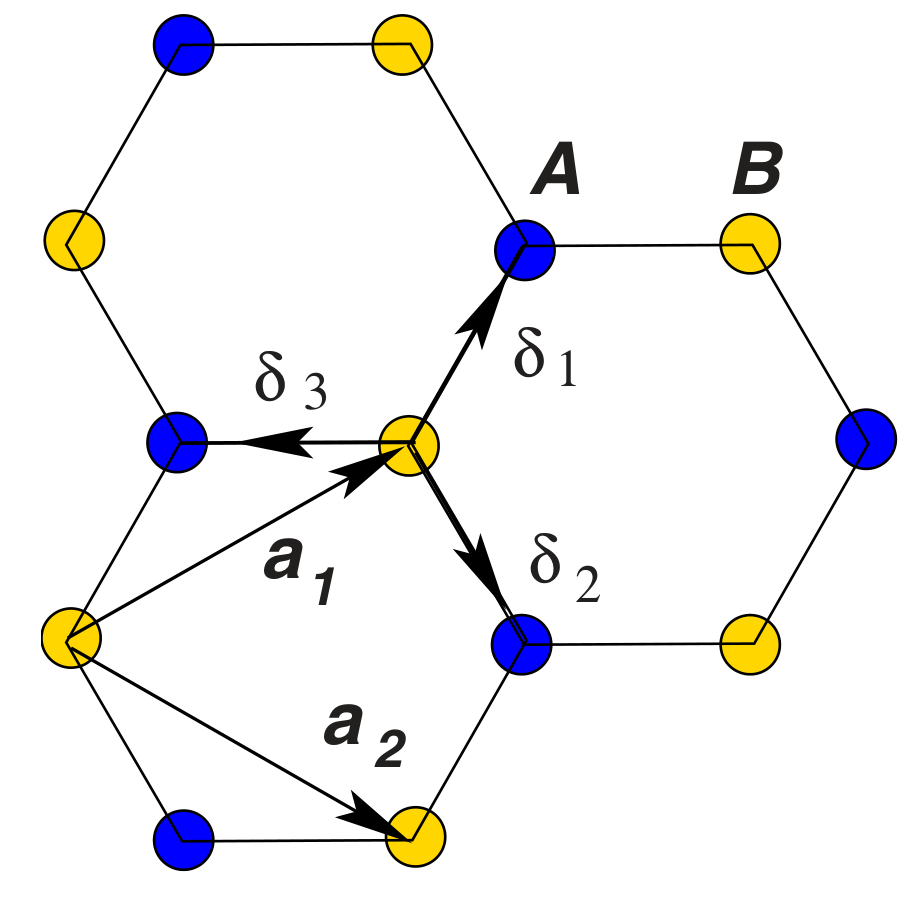
\includegraphics[width=0.3\linewidth]{fig/graphene-lattice_vectors.png}
\label{fig:graphene-lattice_vectors}
\caption{Graphene lattice vectors. Taken from \cite{geim}}
\end{figure}

The lattice vectors are $\vb{a}_1 = \frac{a}{2} (3, \sqrt{3})$, $\vb{a}_2 = \frac{a}{2} (3, -\sqrt{3})$ and the three nearest-neighbor vectors are $\bm{\delta}_1 = \frac{a}{2} (1, \sqrt{3})$, $\bm{\delta}_2 = \frac{a}{2} (1, -\sqrt{3})$, and $\bm{\delta}_3 = a (-1, 0)$.

We write a tight-binding hamiltonian with only nearest-neighbor hopping
$$
H = -t \sum_{i,\nu} \qty(a^\d_{\r_i} b_{\r_i + \bm{\delta}_\nu} + h.c. ),
$$
where $\r_i$ runs through all sublattice $A$ sites, and $\nu = 1, 2, 3$. Applying the Fourier transforms
$$
a_{\r_i}^\d = \frac{1}{\sqrt{N}} \sum_{\k \in \text{BZ}} e^{-i \k \vdot \r_i} a_{\k}^\d,
$$
$$
b_{\r_i} = \frac{1}{\sqrt{N}} \sum_{\k \in \text{BZ}} e^{i \k \vdot \r_i} b_{\k},
$$
we get
$$
H = \sum_{\k}
\begin{pmatrix}
a_{\k}^\d & b_{\k}^\d
\end{pmatrix}
\begin{pmatrix}
0 & -t f(\k) \\
-t f^*(\k) & 0
\end{pmatrix}
\begin{pmatrix}
a_{\k} \\ b_{\k}
\end{pmatrix},
$$
with
$$
f(\k) = \sum_{\nu} e^{i \k \vdot \bm{\delta}_\nu} =
e^{-i k_x a} \qty[ 1 + 2 e^{-3ik_x a / 2} \cos(\sqrt{3} k_y a / 2) ].
$$

The eigenenergies of $h_{\k}$ (UNDEFINED yet) are $E_\pm(\k) = \pm t \abs{f(\k)}$.

The roots of $f(\k)$ are given by solving $f(\k) = 0$, which gives us
$$
2 e^{-3ik_x a / 2} \cos(\sqrt{3} k_y a / 2) = -1 \implies
\begin{cases}
\; e^{-3i k_x a/2} = - 1, \\
\; \cos(\sqrt{3} k_y a / 2) = \frac{1}{2}.
\end{cases}
\implies
\begin{cases}
\; k_x = \frac{2\pi}{3a}, \\
\; k_y = \pm \frac{2\pi}{3 \sqrt{3} a},
\end{cases}
$$
Therefore we define
$$
\K = \frac{2\pi}{3a} \qty(1, \frac{\sqrt{3}}{3}) \; \text{ and } \;
\K' = \frac{2\pi}{3a} \qty(1, -\frac{\sqrt{3}}{3})
$$
which are the so-called Dirac points, around which the dispersion relation are approximately linear $E(\K + \q) = v_F \abs{\q} + O\qty[(\frac{q}{K})^2]$.

%%-----
%% Referências bibliográficas
%%-----
\addcontentsline{toc}{chapter}{\bibname}
%\bibliographystyle{abntex2-num}
\bibliography{citations}
\bibliographystyle{ieeetr}


\end{document}
